% !TEX root = presentation.tex
\section{Background}
\subsection{Mutation Testing Overview}
\frame{\frametitle{Mutation Testing Overview}
  \begin{figure}[!tb]
    \centering
    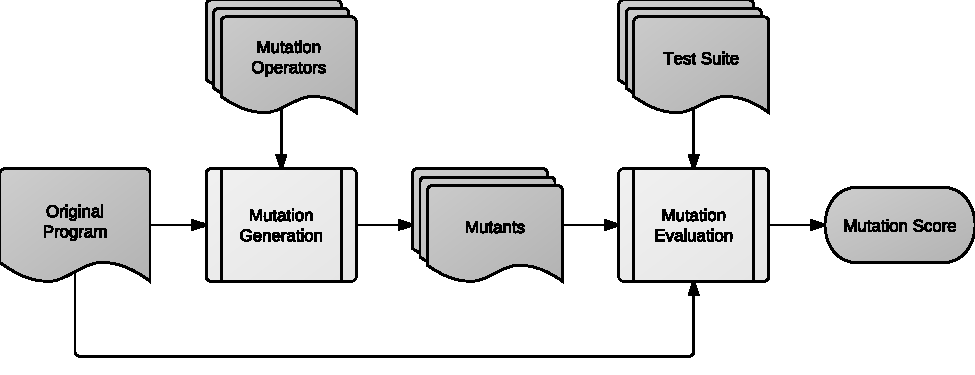
\includegraphics[width=\textwidth]{../thesis/figures/mutation_testing_overview.pdf}
    \caption{The mutation testing process.}
    \label{fig:mutation_testing_overview}
  \end{figure}
  \hrule
  \vspace{5mm}
  \begin{equation}
    \textit{$\text{mutation score} = \frac{\text{killed mutants}}{\text{total mutants} - \text{equivalent mutants}}$}
    \label{equ:mutation_score}
  \end{equation}
}

\subsubsection{Supporting Mutation Testing}
\frame{\frametitle{Supporting Mutation Testing}
  \begin{itemize}
    \item \textit{Competent Programmer Hypothesis}~\footcite{ABD+79}: developers write software that is nearly correct.
    \item \textit{Coupling Effect Hypothesis}~\footcite{Off92}: a large percent of complex faults can be detected if all the simple faults can be detected.
    \item Together these two hypothesis strengthen:
    \begin{itemize}
      \item The use of small/single changes for mutation operators.
      \item Why mutation testing is adequate for evaluating test suite effectiveness.
    \end{itemize}
  \end{itemize}
}

\subsubsection{Method-Level Mutation Operators}
\frame{\frametitle{Method-Level Mutation Operators}
  \scriptsize
  \begin{table}[!tb]
    \centering
    \rowcolors{2}{gray!30}{gray!20}
    \begin{tabular}{|l|l|}
      \hline
      \rowcolor[RGB]{169,196,223}
      \textbf{Operator} & \textbf{Description} \\
      \hline \textit{AOR} & Arithmetic Operator Replacement \\
      \hline \textit{AOI} & Arithmetic Operator Insertion \\
      \hline \textit{AOD} & Arithmetic Operator Deletion \\
      \hline \textit{ROR} & Relational Operator Replacement \\
      \hline \textit{COR} & Conditional Operator Replacement \\
      \hline \textit{COI} & Conditional Operator Insertion \\
      \hline \textit{COD} & Conditional Operator Deletion \\
      \hline \textit{SOR} & Shift Operator Replacement \\
      \hline \textit{LOR} & Logical Operator Replacement \\
      \hline \textit{LOI} & Logical Operator Insertion \\
      \hline \textit{LOD} & Logical Operator Deletion \\
      \hline \textit{ASR} & Assignment Operator Replacement \\
      \hline
    \end{tabular}
    \caption{The set of method-level mutation operators from the \textit{MuJava} mutation testing tool~\footcite{MOK05}.}
    \label{tab:method_operators}
  \end{table}
}

\subsubsection{Mutation Operator Example (ROR)}
\frame{\frametitle{Mutation Operator Example (\textit{ROR})}
  \begin{figure}[!tb]
    \centering
    \begin{minipage}{4.75cm}
      \centering
      \footnotesize{\textbf{Original Program}}
      \lstinputlisting[language=Java, literate={>}{{\textcolor{red}{>}}}{1}]{../thesis/listings/mutation_example.java}
    \end{minipage}
    $\xrightarrow{\textit{ROR}}$
    \begin{minipage}{4.75cm}
      \centering
      \footnotesize{\textbf{Mutant Program}}
      \lstinputlisting[language=Java, literate={>}{{\textcolor{red}{<}}}{1}]{../thesis/listings/mutation_example.java}
    \end{minipage}
    \caption{Example application of the \textit{ROR} method-level mutation operator.}
    \vspace{2mm}
    \hrule
    \label{fig:ROR_mutation}
  \end{figure}
  \begin{itemize}
    \item Replaces a relational operator (i.e., \texttt{>}, \texttt{>=}, \texttt{==}, \texttt{!=}, \texttt{=<} or \texttt{<}) with another type of relational operator.
  \end{itemize}
}

\subsection{Machine Learning}
\frame{\frametitle{Machine Learning}
  \begin{itemize}
    \item Machine learning is a branch of artificial intelligence.
    \item Focuses on the ability to classify complex data.
    \item Uncover patterns that characterize the data.
  \end{itemize}
}

\subsubsection{Machine Learning Categories}
\frame{\frametitle{Machine Learning Categories}
  \begin{itemize}
    \item \textbf{Unsupervised Learning}
    \begin{itemize}
      \item Data has no known category.
      \item Groups data into clusters based on similarity.
    \end{itemize}
    \item \textbf{Supervised Learning}
    \begin{itemize}
      \item Data has known category.
      \item Uses known data (i.e., training data) to predict on unknown data (i.e., test data).
      \item Useful for classification/prediction.
    \end{itemize}
  \end{itemize}
}

\subsubsection{Evaluating Applications of Machine Learning}
\frame{\frametitle{Evaluating Applications of Machine Learning}
  \begin{itemize}
    \item How do you measure the performance of your clustering/classification algorithm?
    \begin{itemize}
      \item Have known data (i.e., the categories are known).
      \item Compare determined category vs. known category.
      \item Use a confusion matrix.
      \item Use known measures.
      \item Use cross-validation (only with supervised learning).
    \end{itemize}
  \end{itemize}
}

\subsubsection{Confusion Matrix}
\frame{\frametitle{Confusion Matrix}
  \begin{figure}[!tb]
    \centering
    \begin{tikzpicture}[
    box/.style={draw,rectangle,minimum size=1.75cm,text width=4.0cm,align=center}]
      \matrix (confusion_matrix) {
        \node (actual_positive_prediction_positive)
        [box,
          label=left:\texttt{A},
          label=above:\texttt{A}
        ] {\underline{True Positives (tp)} \\ \small{\texttt{A} correctly classified as \texttt{A}}};
        \pgfmatrixnextcell
        \node (actual_positive_prediction_negative)
        [box,
          label=above:\texttt{B}
        ] {\underline{False Negatives (fn)} \\ \small{\texttt{A} incorrectly classified as \texttt{B}}};
        \\
        \node (actual_negative_prediction_positive)
        [box,
          label=left:\texttt{B}
        ] {\underline{False Positives (fp)} \\ \small{\texttt{B} incorrectly classified as \texttt{A}}};
        \pgfmatrixnextcell
        \node (actual_negative_prediction_negative)
        [box] {\underline{True Negatives (tn)} \\ \small{reminding categories correctly classified not as \texttt{A}}};
        \\
      };
      \node [left=-.1cm of confusion_matrix,text width=1.5cm,align=right] {\textbf{Actual \\ Value}};
      \node [above=-.1cm of confusion_matrix] {\textbf{Prediction Value}};
    \end{tikzpicture}
    \caption{A $2~\times~2$ confusion matrix for classification results of the \texttt{A} category.}
    \vspace{1mm}
    \footnotesize{\textit{It is possible to extend a confusion matrix to $n~\times~n$ dimensions. For each category the (tp, fn, fp, and tn) variables need to be calculated.}}
    \label{fig:example_confusion_matrix}
  \end{figure}
}

\subsubsection{Machine Learning Performance Measures}
\frame{\frametitle{Machine Learning Performance Measures}
  \begin{itemize}
    \item \textbf{Accuracy} represents the fraction of all true predictions made that were correctly identified.
    \begin{equation}
      \textit{$\text{accuracy} = \frac{TP + TN}{TP + FP + FN + TN}$}
      \label{equ:accuracy}
    \end{equation}
    \item Other traditional performance measures:
    \begin{itemize}
      \item Precision.
      \item Recall.
      \item Specificity.
     \end{itemize}
    \item More sophisticated performance measures:
    \begin{itemize}
      \item F-score.
      \item Balanced Accuracy.
      \item Youden's Index.
     \end{itemize}
  \end{itemize}
}

\subsection{Support Vector Machine}
\frame{\frametitle{Support Vector Machine}
  \begin{itemize}
    \item A supervised machine learning classification technique.
    \item Models a feature space constructed using a set of vectors.
    \item Each vectors has a set of attributes and a category.
    \item Attempts to linearly separate vectors using a hyperplane.
  \end{itemize}
  \begin{figure}
    \centering
    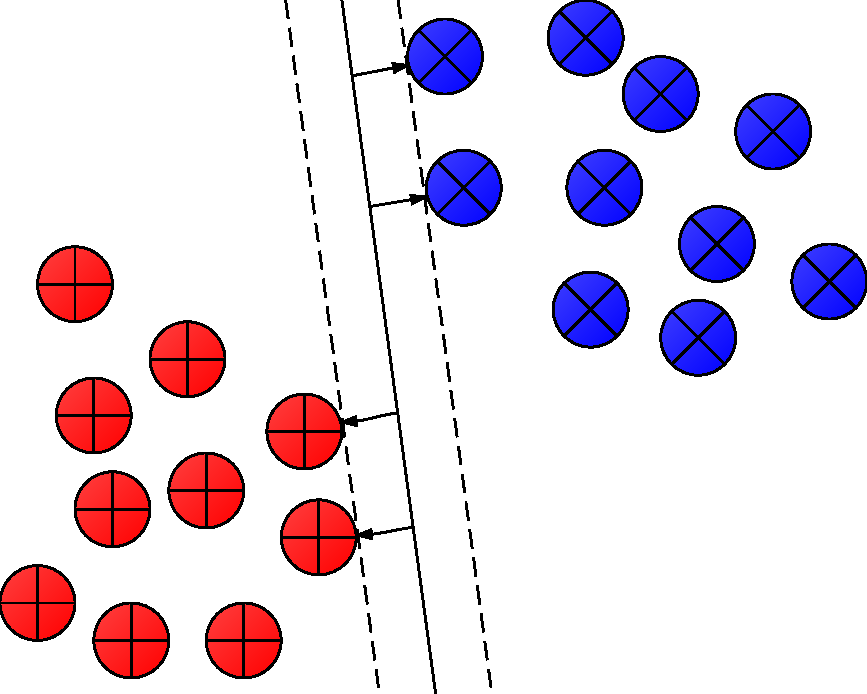
\includegraphics[width=3.5cm]{../thesis/figures/SVM_small_margin.pdf}
    $\xrightarrow{\texttt{Better Margin}}$
    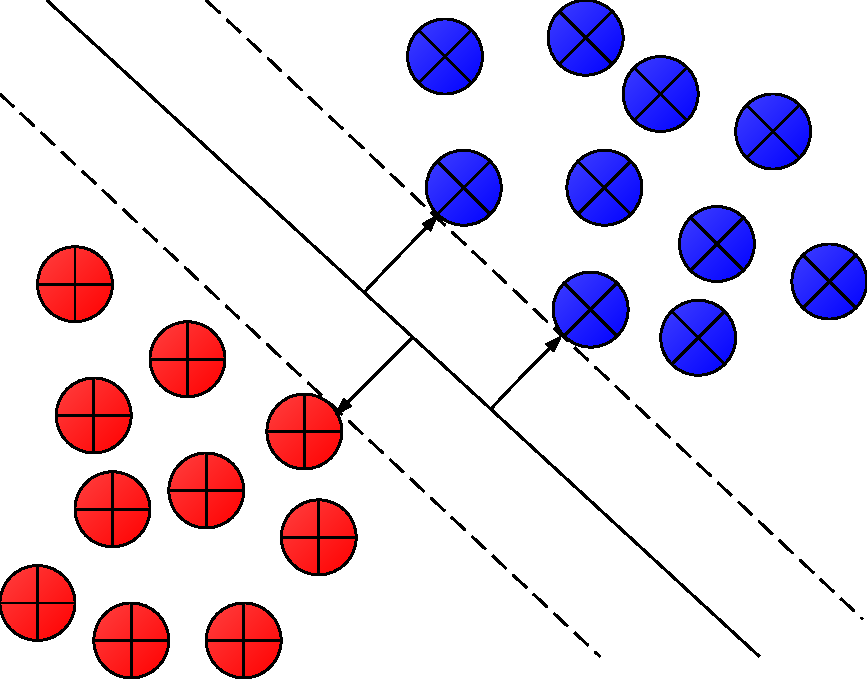
\includegraphics[width=3.5cm]{../thesis/figures/SVM_maximum_margin.pdf}
  \end{figure}
}

\subsubsection{Support Vector Machine Kernel Function}
\frame{\frametitle{Support Vector Machine Kernel Function}
  \begin{itemize}
    \item Can work for \textit{many}-group classification.
    \item Can work on non-linearly separable data using kernel functions.
  \end{itemize}
  \begin{figure}
    \centering
    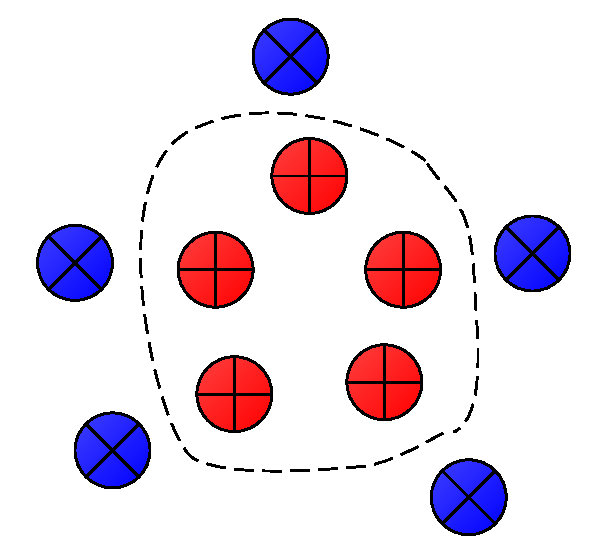
\includegraphics[width=3.5cm]{../thesis/figures/SVM_non-linear.pdf}
    $\xrightarrow{\texttt{Kernel Function}}$
    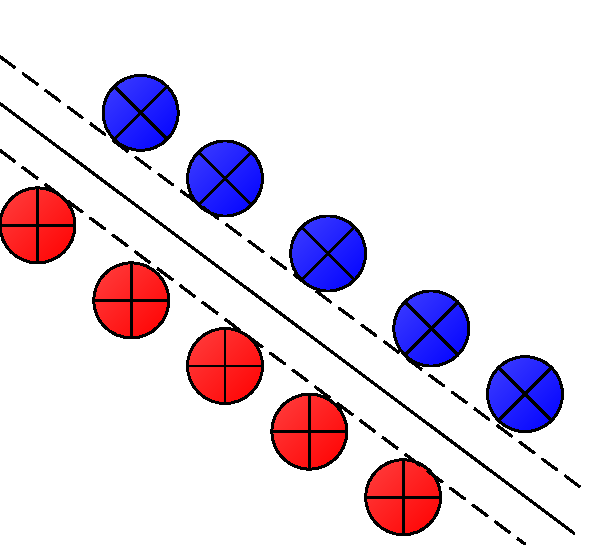
\includegraphics[width=3.5cm]{../thesis/figures/SVM_kernel_function.pdf}
  \end{figure}
}

\subsection{Software Metrics}
\frame{\frametitle{Software Metrics}
  \begin{itemize}
    \item A software metrics can be broken down into the following~\footcite{Fen94}:
    \begin{itemize}
      \item \textbf{Entity:} Represents an object or event.
      \item \textbf{Attribute:} Represents a feature or property of an \textit{entity}.
      \item \textbf{Model:} Represents a specific viewpoint of an \textit{attribute}.
    \end{itemize}
  \end{itemize}
}

\subsubsection{Source Code Metrics}
\frame{\frametitle{Source Code Metrics}
  \begin{itemize}
    \item Measures structural aspects of the source code.
    \item Typically done using static analysis on the source code files.
    \begin{itemize}
      \item Complexity.
      \item Number of source lines of code.
      \item Maximum nested block depth in a method.
      \item Number of methods/classes.
      \item etc\ldots
    \end{itemize}
  \end{itemize}
}

\subsubsection{Test Suite Metrics}
\frame{\frametitle{Test Suite Metrics Metrics}
  \begin{itemize}
    \item Measures structural aspects of the test suite typically using static analysis.
    \begin{itemize}
      \item Similar to source code metrics (e.g., complexity, etc\ldots).
    \end{itemize}
    \item Measures relationship between test suite and the software system under test.
    \begin{itemize}
      \item Number of test cases for system/class/method.
      \item Statement/branch/decision coverage.
    \end{itemize}
  \end{itemize}
}
